\documentclass[sigconf]{acmart}

\usepackage{clrscode3e}
\usepackage{tabularx}

% Copyright
%\setcopyright{none}
\setcopyright{acmcopyright}
%\setcopyright{acmlicensed}
%\setcopyright{rightsretained}
%\setcopyright{usgov}
%\setcopyright{usgovmixed}
%\setcopyright{cagov}
%\setcopyright{cagovmixed}

% DOI
%\acmDOI{10.475/123_4}

% ISBN
%\acmISBN{123-4567-24-567/08/06}

%Conference
%\acmConference[WOODSTOCK'97]{ACM Woodstock %conference}{July 1997}{El
%  Paso, Texas USA} 
%\acmYear{1997}
%\copyrightyear{2016}

%\acmArticle{4}
%\acmPrice{15.00}

% These commands are optional
%\acmBooktitle{Transactions of the ACM Woodstock conference}
%\editor{Jennifer B. Sartor}
%\editor{Theo D'Hondt}
%\editor{Wolfgang De Meuter}

\begin{document}
\title{StarCraft AI Research Summary}
%\titlenote{}
%\subtitle{}
%\subtitlenote{}

\author{Qinyu Chen}
%\authornote{}
%\orcid{}
\affiliation{%
  \institution{}
  \streetaddress{}
  \city{BeiJing} 
  \state{China} 
  \postcode{}
}
\email{henryqychen@gmail.com}

\begin{abstract}
This paper provides a sample of a \LaTeX\ document which conforms, somewhat loosely, to the formatting guidelines for
ACM SIG Proceedings.
%\footnote{This is an abstract footnote}
\end{abstract}

\keywords{StarCraft, Reinforcement Learning, Inperfect Information Game, Exploration and Exploitation, Markov Decision Process, Generative Adversarial Networks}

\maketitle

%------------------------------

\section{Introduction}
\subsection{The Game}
\textbf{StarCraft$^\circledR$} is a famous military science fiction real-time strategy video game developed and published by \textbf{Blizzard Entertainment$^\circledR$} in 1998.
\subsection{Why Choose StarCraft for AI Research}
StarCraft has proven to be a challenging environment for artificial intelligence research. While hand-crafted strategies are still the state-of-art, the deep networks approach is able to express a wide range of different strategies and thus improving the network’s performance with deep reinforcement learning is an immediately promising avenue for future research.\cite{DBLP:journals/corr/JustesenR17}
\subsubsection{Advantages}
\begin{itemize}
\item Large-scale game replays data in communities
\item Game with perfect designed balance, competitiveness and purity
\end{itemize}

\subsubsection{Challenges}
\begin{itemize}
\item Enormous Search Space(10 times complexer than \emph{Go} by game states and actions)
\item Partially observed environment
\item Memory preserving agent
\item Inference both in time and space
\item Multi-agent corporation
\item High time efficiency engineering
\end{itemize}

\subsection{Online Resources}
\subsubsection{Replays}
\begin{itemize}
\item \emph{GosuGamers}
	  \footnote{\url{http://www.gosugamers.net}}
\item \emph{ICCup}
	  \footnote{\url{https://iccup.com}}
\item \emph{TeamLiquid}
	  \footnote{\url{http://www.teamliquid.net}}
\end{itemize}
\subsubsection{Competitions}
\begin{itemize}
\item \emph{AIIDE StarCraft AI Competition}
	  \footnote{\url{https://sites.google.com/view/aiide2017}}
\item \emph{CIG StarCraft RTS AI Competition}
	  \footnote{\url{https://ls11-www.cs.tu-dortmund.de/rts-competition/start}}
\item \emph{Student StarCraft AI Competition}
	  \footnote{\url{https://sscaitournament.com}}
\end{itemize}

\section{Game AI}
\subsection{Thread in Game AI}
Usually there is only one thread to handle AI logic, otherwise there could be multi-threaded for computation and one thread for rendering.
\subsection{Difficulty Level of Game AI design}
The most difficult AI design is for sports game, which is very similar to robotics.
\begin{eqnarray*}
MMO<FPS<RTS<Sports
\end{eqnarray*}

\subsection{Traditional Game AI Methods}
\subsubsection{State Machine}
\subsubsection{Hierarchical State Machine}
\subsubsection{Behavior Tree}

\section{RTS Game AI}
Real-time strategy (RTS) games have historaically been a domain of interest of the planning and decision making research communities.
\subsection{Macromanagement AI}
Or General's AI, which determine the time series of constructing buildings, conducting research, and producing units, among other things involving the intake and expending of resources. This is actually a form of micromanagement done to a relatively large number of units
\subsubsection{Rule-based methods}
Implemented by if-else.
\begin{itemize}
\item TODO
\end{itemize}

\subsubsection{Advanced methods}
\begin{itemize}
\item planner
\item scoring system, power map
\item machine learning methods
\end{itemize}

\subsection{Agent AI}
Or Soldier's AI, human player's micro-operation.

\subsubsection{State Machine}
Behaviors will be triggered in certain condition(environment, resource, time)

\subsubsection{Behavior Tree}
Theoretically, the behavior tree is equivalent to state machine but could reduce the complexity of control logic.\\
Practically, behavior tree need only 1/3 lines of more readable code  comparing with the same logic implemented by FSM.

\subsubsection{Hierarchical State Machine}
This is a traditional and efficient method to reduce the complexity of game AI design.

\section{Modeling RTS Game}
\subsection{Reinforcement Learning Framework}
Reinforcement Learning (RL) is an area of machine learning inspired by behaviourist psychology, concerned with how agents should take actions in an environment so as to maximize cumulative reward.\\
There are four main reasons that make RL quite different from other machine learning paradigms:\cite{David_Silver:intro_RL}
\begin{itemize}
\item Unlike supervised-learning, there is no supervisor, only a reward signal
\item Unlike online-learning, the feedback is delayed, not instantaneous
\item The data is sequential (non i.i.d data), time really matters
\item Agents' actions affect the subsequent data it receives
\end{itemize}
RL focus on online performance, which involves finding a balance between exploration (of uncharted territory) and exploitation (of current knowledge). The $E\&E$ trade-off in RL has been most thoroughly studied through the multi-armed bandit (MAB) problem and in finite MDPs.

\begin{table}[htb]
\caption{Formal Definition of Reinforcement Learning\cite{David_Silver:intro_RL}}
\centering
\begin{tabularx}{0.45\textwidth}{cX}
\hline Symbols & Discription \\ \hline
$a$ & \emph{Agent} \\
$e$ & \emph{Environment} \\
$t$ & \emph{Timestamp}, increments at each step \\
$O_t$ & agent's \emph{Observation} (input) from environment at step $t$ \\
$A_t$ & agent's \emph{Actions} (output) to environment at step $t$ \\
$R_t$ & agent's \emph{Reward} at step $t$, a scalar feedback signal\\
$S_t^a$ & \emph{Agent's State} at step $t$ \\
$S_t^e$ & \emph{Environment's State} at step $t$ \\
$\pi$ & Given a state $s$ at step $t$, \emph{Policy} is the probability of agent's choice of action $a$,
$\pi(a \mid s)=\mathbb{P}[A_t=a \mid S_t = s]$ \\
$\mathcal{P}$ & Given a state $s$ and an action $a$ at step $t$, the model predicts the probability of next state $s'$, $\mathcal{P}_{ss'}^a =\mathbb{P}[S_{t+1}=s' \mid S_t=s, A_t=a]$ \\
$\mathcal{R}$ & Given a state $s$ and an action $a$ at step $t$, the model predicts the expection of next reward, $\mathcal{R}_{s}^a =\mathbb{E}[R_{t+1} \mid S_t=s, A_t=a]$ \\
$v$ & \emph{Value Function} is a prediction of expected future reward to evaluate the goodness/badness of states,
$v_\pi(s)=\mathbb{E}_\pi[\sum\limits_{i=0}^{+\infty}\gamma^{i}R_{t+i+1} \mid S_t=s]$
\end{tabularx}
\label{table:formal_definition_of_RL}
\end{table}

\subsection{Inperfect Information Game}
In full observability game, agent directly observes the environment stat, where:
\begin{eqnarray}
O_{t}^a = S_{t}^a = S_{t}^e
\end{eqnarray}
As mentioned in 1.2.2, because of the game mechanisms: \emph{fog-of-war} and confusing magic (invisibility, hallucination, etc.), agents receive inperfect information from partially observed environment.
\begin{eqnarray}
S_{1,t}^{a} \neq S_{2,t}^{a} \\
S_{1,t}^{a} \cup S_{2,t}^{a} = S_t^e
\end{eqnarray}

\begin{figure}[htb]
\centering
\caption{1v1 Adversarial RL Framework}
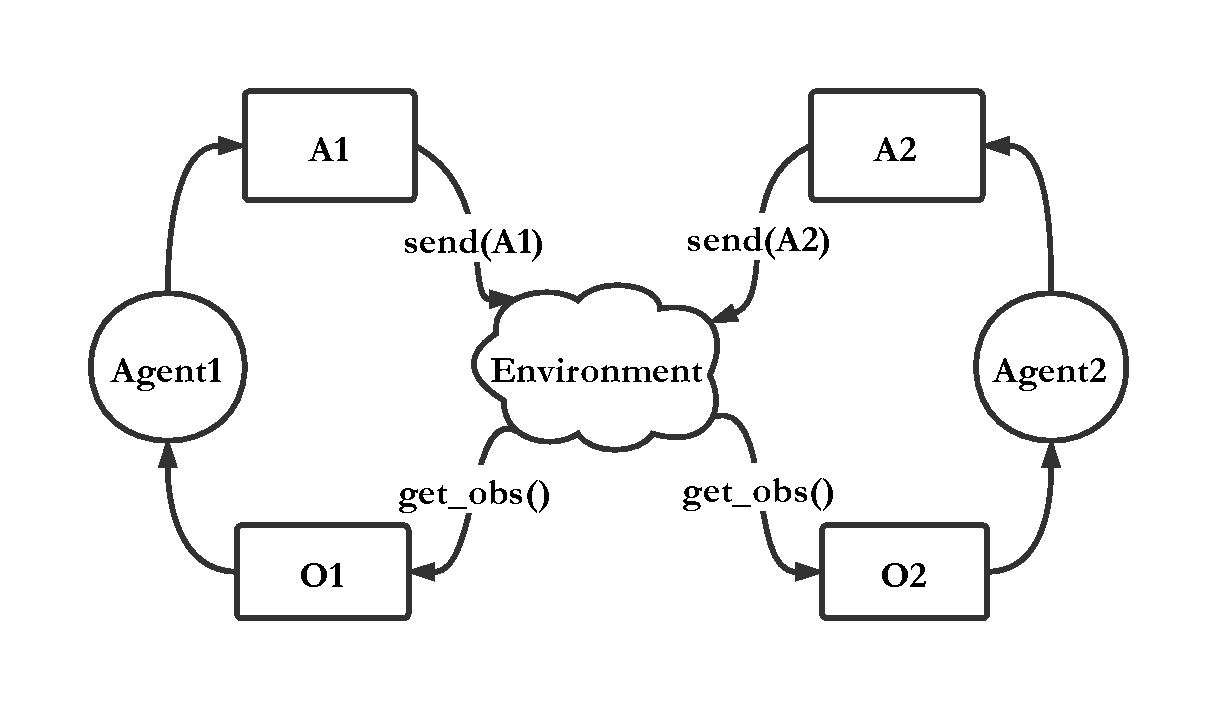
\includegraphics[width=0.35\textwidth]{./img/Adversarial_Reinforcement_Learning.pdf}
\end{figure}

\section{Developing Environment}
\subsection{Tools}
\subsubsection{BWAPI}
The Brood War Application Programming Interface (BWAPI) is a free and open source C++ framework used to interact with \textbf{Starcraft: BroodWar$^\circledR$}. Researchers can create AI agents to play the game.\cite{GitHub:bwapi}
\subsubsection{Torch}
\emph{Torch} is a scientific computing framework with wide support for machine learning algorithms that puts GPUs first.
Torch is mainly implemented by \emph{LuaJIT}.\cite{GitHub:torch}
\subsubsection{TorchCraft}
\emph{TorchCraft} is a bridge between Torch and StarCraft.\cite{GitHub:TorchCraft,DBLP:journals/corr/SynnaeveNACLLRU16}
\subsubsection{TorchCraft-Py}
A Python wrapper for TorchCraft developed by Alibaba.\cite{GitHub:torchcraft-py}
\subsubsection{gym}
An open source reinforcement framework
\subsubsection{gym-starcraft}

\subsection{Architecture}
\begin{figure}[htb]
\caption{TorchCraft-based Client-Server Architecture}
\centering
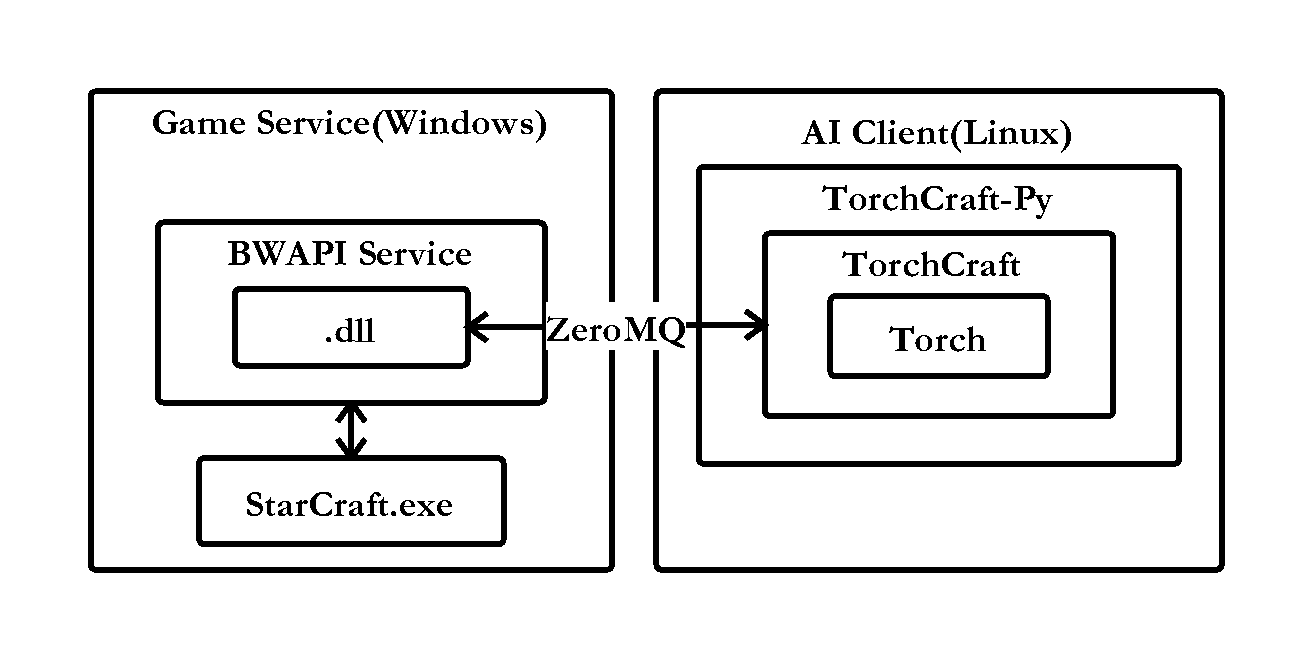
\includegraphics[width=0.45\textwidth]{./img/Client_Server_Architecture.pdf}
\end{figure}

\subsection{BWAPI}
\subsubsection{Client}
\subsubsection{ServerState}
\subsubsection{Frame}
\paragraph{Order}
\paragraph{Unit}
\paragraph{Resources}
\paragraph{Bullet}
\paragraph{Action}

\section{Macromanagement AI}
\subsection{Build Order Planning}
\subsubsection{Search Problem}
the goal is to find the build order that optimizes a specific heuristic.
\paragraph{Notes and Comments.}
\subsection{Dataset}
\subsubsection{Format}
Replay files are in binary format and require preprocessing before knowledge can be extracted.
\subsection{Learning from replays}

\subsection{}

\begin{codebox}
\Procname{Algorithm 2: $\proc{Insertion-Sort}(A)$}
\li \For $j \gets 2$ \To $\attrib{A}{length}$
\li \Do
$\id{key} \gets A[j]$
\li \Comment Insert $A[j]$ into the sorted sequence
$A[1 \twodots j-1]$.
\li $i \gets j-1$
\li \While $i > 0$ and $A[i] > \id{key}$
\li \Do
$A[i+1] \gets A[i]$
\li $i \gets i-1$
\End
\li $A[i+1] \gets \id{key}$
\End
\end{codebox}

\section{Micromanagement AI}
\subsection{}

%------------------------------

\bibliographystyle{unsrt}
\bibliography{starcraft}

\end{document}
